\chapter{XPATH}
\section{XML in Memory}
XML is text-based but while in memory, is stored as a tree. There are different ways to access these trees:
\begin{itemize}
	\item DOM (document object model):
	The default HTML-Version but if possible, other ways should be used.
	\item XQuery and XPath data model (XDM):
	More powerful than DOM, easier to access data as objects.
	\item post-schema validation information set (PSVI):
	XML Schema's own version.
\end{itemize}

\section{DOM}
DOM contains of different nodes, the most important ones being document nodes, element nodes, attribute nodes and text nodes.
DOM provides only a low level API to access its objects in the tree. DOM is known to be inefficient when compared to XPath and only offers basic object-oriented features.

\section{XPath}
XPath can be used to select and point into XML documents. There are API's for all major programming languages available.
Usually, one XML-file and a XPath-expression are fed into a XPath engine which then returns a node list.
\subsection{XPath Axes}
An XPath axis is a direction and each / stands for a step you move along this axis. There are also other commands which are listed below:\\
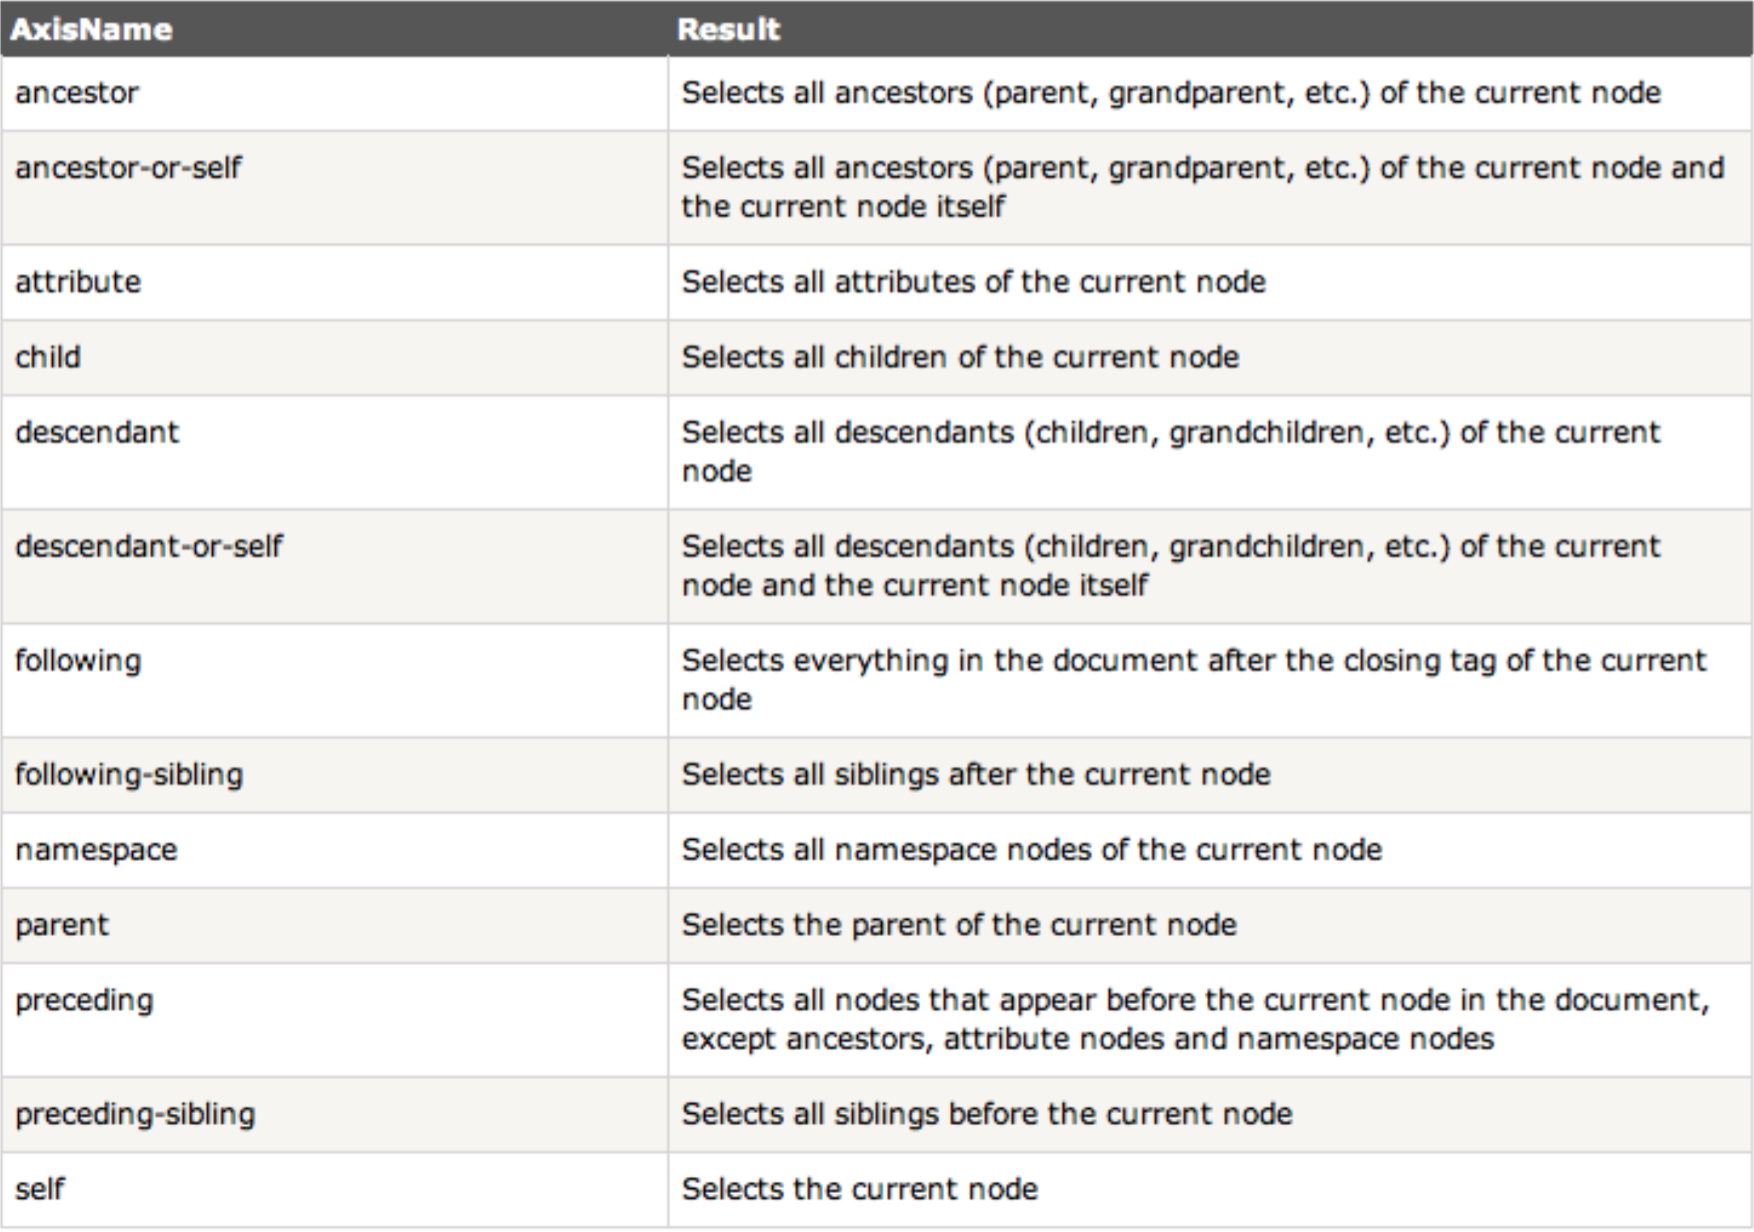
\includegraphics[width=\textwidth]{fig/XPathAxes.png}
Further selection is possible using other XPath expressions:
\begin{itemize}
	\item text(): to access the text of the selected node
	\item $\lbrack$@attribute$\rbrack$: applying a filter on the selection
	\item $\lbrack$number$\rbrack$: returns the element at number
\end{itemize}

\section{Exercises 1}
\begin{enumerate}
\item Make a prediction what the following expression returns and verify
\begin{lstlisting}[language=XML]
/descendant::title[text() = "Dr. No"]/../regie
\end{lstlisting}

\item Which number has the Bond movie with Maud Adams ?
\begin{enumerate}
\item solve the exercise with knowledge that she was a Bond Girl.
\begin{lstlisting}[language=XML]
//bond_girl[text() = "Maud Adams"]/../@number
\end{lstlisting}
\item solve it without knowing that she was a Bond Girl
\begin{lstlisting}[language=XML]
//*[text() = "Maud Adams"]/../@number
\end{lstlisting}
\end{enumerate}
\item How many times (use $count()$) did Sean Connery play Bond ?
\begin{lstlisting}[language=XML]
count(//bond[text() = "Sean Connery"])
\end{lstlisting}

\item My friends and I plan a James Bond movie night where we want to watch all movies from the very first to the very last.
How much time (use $sum()$) will this take ?
\begin{lstlisting}[language=XML]
sum(//duration)
\end{lstlisting}

\item List all movies over 120min
\begin{lstlisting}[language=XML]
//duration[text()>120]/../title
\end{lstlisting}

\item List all Bond actors without double naming (use distinct-values())
\begin{lstlisting}[language=XML]
distinct-values(//bond)
\end{lstlisting}
\end{enumerate}

\section{XPath variables and conditional queries}
Variables can be configured using the prefix \$ and can be used as following:
\begin{lstlisting}[language=XML]
for $i in distinct-values(/descendant::bond)
return concat($i, " played ", count(/bond_movies/movie[bond = $i]), " times.")
\end{lstlisting}

Conditional statements have to be implemented like this:
\begin{lstlisting}[language=XML]
if(count(/bond_movies/movie[regie = "John Glen"]) > 1)
 then "There is more than one from this director"
 else "There is exactly one movie from this director"
\end{lstlisting}


\section{Exercises 2}
\begin{enumerate}
\item Formulate an XPath query that produces the following output. (<<regie>> produced <<count()>> movies)
\begin{lstlisting}[language=XML]
for $i in distinct-values(/descendant::regie)
return concat($i, " produced ",
count(/bond_movies/movie[regie = $i]), " movies.")
\end{lstlisting}

\item Modify that it shows only regisseurs with more than one movie produced
\begin{lstlisting}[language=XML]
for $i in distinct-values(/descendant::regie)
return if(count(/bond_movies/movie[regie = $i])>1) then
concat($i, " produced ",
count(/bond_movies/movie[regie = $i]), " movies.")
else()
\end{lstlisting}
\end{enumerate}

\section{More XPath Exercises}
Generate for the following XML:
\begin{center}
\begin{lstlisting}[language=XML]
<?xml version="1.0" ?>
<european_countries year="2012">
	<country code="CH">
		<name>Switzerland</name>
		<population>8139600</population>
		<population_under_15>14.8</population_under_15>
		<population_over_64>17.4</population_over_64>
		<life_exp_men>80.0</life_exp_men>
		<life_exp_women>84.7</life_exp_women>
	</country>
	<country code="DE">
		<name>Germany</name>
		<population>81890000</population>
		<population_under_15>13.1</population_under_15>
		<population_over_64>20.7</population_over_64>
		<life_exp_men>78.0</life_exp_men>
		<life_exp_women>82.7</life_exp_women>
	</country>
	<country code="A">
		<name>Austria</name>
		<population>8462000</population>
		<population_under_15>14.5</population_under_15>
		<population_over_64>18.1</population_over_64>
		<life_exp_men>77.1</life_exp_men>
		<life_exp_women>83.1</life_exp_women>
	</country>
	<country code="F">
		<name>France</name>
		<population>65697000</population>
		<population_under_15>18.2</population_under_15>
		<population_over_64>17.6</population_over_64>
		<life_exp_men>78.5</life_exp_men>
		<life_exp_women>84.8</life_exp_women>
	</country>
	<country code="I">
		<name>Italy</name>
		<population>60918000</population>
		<population_under_15>14.1</population_under_15>
		<population_over_64>21.2</population_over_64>
		<life_exp_men>79.3</life_exp_men>
		<life_exp_women>84.7</life_exp_women>
	</country>
	<country code="E">
		<name>Spain</name>
		<population>46218000</population>
		<population_under_15>15.4</population_under_15>
		<population_over_64>17.7</population_over_64>
		<life_exp_men>78.4</life_exp_men>
		<life_exp_women>84.6</life_exp_women>
	</country>
	<country code="GR">
		<name>Greece</name>
		<population>11280000</population>
		<population_under_15>14.6</population_under_15>
		<population_over_64>20.1</population_over_64>
		<life_exp_men>77.6</life_exp_men>
		<life_exp_women>82.9</life_exp_women>
	</country>
	<country code="NL">
		<name>Netherlands</name>
		<population>16768000</population>
		<population_under_15>17.1</population_under_15>
		<population_over_64>16.8</population_over_64>
		<life_exp_men>78.9</life_exp_men>
		<life_exp_women>83.2</life_exp_women>
	</country>
	<country code="S">
		<name>Sweden</name>
		<population>9517000</population>
		<population_under_15>16.9</population_under_15>
		<population_over_64>19.1</population_over_64>
		<life_exp_men>79.0</life_exp_men>
		<life_exp_women>83.4</life_exp_women>
	</country>
	<country code="B">
		<name>Belgium</name>
		<population>11142000</population>
		<population_under_15>17.0</population_under_15>
		<population_over_64>17.6</population_over_64>
		<life_exp_men>76.6</life_exp_men>
		<life_exp_women>83.0</life_exp_women>
	</country>
	<country code="L">
		<name>Luxembourg</name>
		<population>531000</population>
		<population_under_15>17.5</population_under_15>
		<population_over_64>14.0</population_over_64>
		<life_exp_men>76.6</life_exp_men>
		<life_exp_women>83.3</life_exp_women>
	</country>
	<country code="IS">
		<name>Iceland</name>
		<population>320000</population>
		<population_under_15>20.7</population_under_15>
		<population_over_64>12.9</population_over_64>
		<life_exp_men>78.9</life_exp_men>
		<life_exp_women>83.4</life_exp_women>
	</country>
	<country code="P">
		<name>Portugal</name>
		<population>10524000</population>
		<population_under_15>14.8</population_under_15>
		<population_over_64>19.4</population_over_64>
		<life_exp_men>75.6</life_exp_men>
		<life_exp_women>82.3</life_exp_women>
	</country>
	<country code="DK">
		<name>Denmark</name>
		<population>5590000</population>
		<population_under_15>17.6</population_under_15>
		<population_over_64>15.7</population_over_64>
		<life_exp_men>76.5</life_exp_men>
		<life_exp_women>81.2</life_exp_women>
	</country>
	<country code="N">
		<name>Norway</name>
		<population>5019000</population>
		<population_under_15>18.4</population_under_15>
		<population_over_64>15.7</population_over_64>
		<life_exp_men>77.8</life_exp_men>
		<life_exp_women>83.2</life_exp_women>
	</country>
	<country code="FIN">
		<name>Finland</name>
		<population>5414000</population>
		<population_under_15>16.4</population_under_15>
		<population_over_64>18.8</population_over_64>
		<life_exp_men>76.0</life_exp_men>
		<life_exp_women>83.2</life_exp_women>
	</country>
	<country code="IRL">
		<name>Ireland</name>
		<population>4589000</population>
		<population_under_15>21.6</population_under_15>
		<population_over_64>12.2</population_over_64>
		<life_exp_men>78.2</life_exp_men>
		<life_exp_women>82.8</life_exp_women>
	</country>
	<country code="GB">
		<name>United Kingdom</name>
		<population>63228000</population>
		<population_under_15>17.6</population_under_15>
		<population_over_64>17.2</population_over_64>
		<life_exp_men>78.2</life_exp_men>
		<life_exp_women>82.5</life_exp_women>
	</country>
</european_countries>
\end{lstlisting}
\end{center}
\begin{enumerate}
\item List all countries with population less than Switzerland
\begin{lstlisting}[language=XML]
for $i in /descendant::name
return if($i/../population/text() > //name[text() = "Switzerland"]/../population/text()) then
$i
else()
\end{lstlisting}

\item List all codes of countries with population less than Switzerland
\begin{lstlisting}[language=XML]
for $i in /descendant::name
return if($i/../population/text() > //name[text() = "Switzerland"]/../population/text())
then
$i/../@code
else()
\end{lstlisting}

\item List all countries whose average life expectance between men and women does not differ by more than 4.5 years
\begin{lstlisting}[language=XML]
for $i in //name
return
if(($i/../life_exp_men - $i/../life_exp_women) < 4.5
and ($i/../life_exp_men - $i/../life_exp_women) > (-4.5))
then
$i/../name
else ()
\end{lstlisting}

\item Find the country with the fewest people
\begin{lstlisting}[language=XML]
//population[not(. > //population)][1]/../name
\end{lstlisting}

\item List all countries with less than 1.5M people under 15 years
\begin{lstlisting}[language=XML]
for $i in //population_under_15
return
if (($i/text() * $i/../population * 0.01)<1500000) then
$i/../name
else ()
\end{lstlisting}

\item Find all countries with at least 50\% more young than old people
\begin{lstlisting}[language=XML]
\end{lstlisting}

\item $\textnormal{Dependency ratio}=\frac{\textnormal{Number of people aged 0-14 and those aged 65 and older}}{\textnormal{number of people aged 15-64}}\times 100$. Generate the following output:\\
Switzerland has dependency ratio 47.4926253687316 \\
Germany has dependency ratio 51.057401812688\\...
\begin{lstlisting}[language=XML]
\end{lstlisting}

\item Generate the following management summary:\\
Switzerland has negative trend\\
Germany has positive trend\\...
\begin{lstlisting}[language=XML]
\end{lstlisting}
\end{enumerate}

\section {Bootcamp XPath}
Geben sie mittels XPath eine Liste aller Spendenaktionen ohne Doppelnennungen aus, für welche 2013 Einzahlungen getätigt wurden, dh. generieren sie folgende Resultatemenge:\\
Ueberschwemmungen Europa\\
Syrienkonflikt\\
Jeder Rappen zaehlt\\
\begin{lstlisting}[language=XML]
	distinct-values(//donation[@year="2013"])
\end{lstlisting}
Geben sie mittels XPath eine Liste aller Spenderdaten aus, die unter anderem einen Eintrag zu Gunsten Orkan Lothar enthalten.
\begin{lstlisting}[language=XML]
	//donation[text()="Orkan Lothar"]/..
\end{lstlisting}
Berechnen sie mittels XPath die Summer der im Jahr 2013 eingegangen Spenden.
\begin{lstlisting}[language=XML]
	sum(//donation[@year="2013"]/[@amount])
\end{lstlisting}
Berechnen sie mittels XPath die Anzahl Privatpersonen, welche im Jahr 2013 mindestens eine Spende getaetigt haben.
\begin{lstlisting}[language=XML]
	count(//donator[desc/text()="Privatperson" and donation/@year="2013"])
	richtig richtige Loesung
	count(//donation/../desc[text()="Privatperson"]/../donation[@year="2013"][1])
\end{lstlisting}
